\section{Baseline Algorithms}
To better measure the performance of our network, we compare it to non-deep learning anomaly detection algorithms. These algorithms come from the Python machine learning framework \gls{scikit-learn} \cite{scikit-learn}. \gls{scikit-learn} provides different alternatives for anomaly detection on 2D datasets. We use the algorithms \gls{iso} and \gls{lof} for baselines to measure our model against, as these show the best results out of the algorithms for anomaly detection found in \gls{scikit-learn} \cite{sklearn-anomaly}. \newline

\noindent
The \gls{scikit-learn} algorithms will be tested on the time series listed in Table \ref{tab:datasets} in order to test our model with the baseline algorithms.

\subsection{Isolation Forest}
\Gls{iso} is an algorithm used to find anomalies using a fast algorithm first described by \cite{isolation_forest}. The idea is that anomalies are few and isolated from the normal points. We can see in Figure \ref{fig:iso} that isolated points generally require fewer cuts to be isolated as the graph to the right exemplifies.

\begin{figure}[htbp]
    \centering
    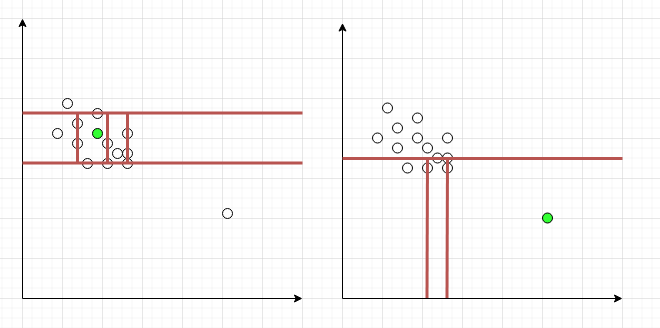
\includegraphics[width=0.9\textwidth]{Pictures/Sprint_4/isolation_forrest.png}
    \caption{Random cuts are performed until the point of interest is isolated (colored green). }
    \label{fig:iso}
\end{figure}

\noindent
The algorithm gives an anomaly score to every point. The point score is given by counting the number of random cuts required to isolate the point from all other points completely. In theory, this count should be lower for anomaly points, as illustrated in Figure \ref{fig:iso}. The algorithm is fast as it removes roughly half the remaining points at each cut.

The recursive nature of the cuts means that it can be represented by a tree structure where the number of cuts is equivalent to the length of a path from the root node to the terminating node. Averaging this path length over multiple random trees results in a better anomaly score\cite{isolation_forest}.

The algorithm is fast and works well on multidimensional data but also suffers from potentially bad accuracy as there can potentially be many false positives, especially if the anomaly threshold is not carefully set.

\subsection{Local Outlier Factor}
\gls{lof} is an algorithm used to find anomalies using an algorithm to find "local" anomalies first described in \cite{lof}. The idea is that anomalies are not only found globally, but also locally in clusters of data.

\begin{figure}[htbp]
    \centering
    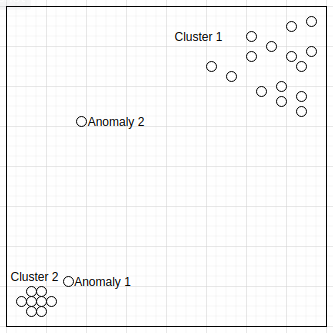
\includegraphics[width=0.4\textwidth]{Pictures/Sprint_4/lof.png}
    \caption{Local anomalies are looked at, instead of global anomalies.}
    \label{fig:lof}
\end{figure}

\noindent 
The algorithm looks for anomalies by looking at how many objects $p$, a specific object $o$, have a distance to less than the distance from $o$ to an object $k$, or the $k$-distance. If an object's distance to the object $o$, is less than the $k$-distance, it is part of the $k$-distance neighborhood of $o$, and part of the $k$-nearest neighbors.

As \gls{lof} has to look at local anomalies, a threshold for density can not be specified. As Figure \ref{fig:lof} shows, Anomaly one would not be considered an anomaly, if the density threshold was set not to specify Cluster one as anomalies. Instead of having a density threshold, it is necessary to compare the densities of different sets of objects. \gls{lof}, therefore, has to determine the density of clusters dynamically.

Because it has to determine the density of clusters dynamically, it is slower than \gls{iso}, but is more accurate in most cases.